%2multibyte Version: 5.50.0.2953 CodePage: 1252
% green
% blue
% orange
% purple
% red
% resets numbering each section

\ifdefined\extendedversion\else
  \PassOptionsToClass{handout}{beamer}
\fi
\documentclass[xcolor=x11names,compress,aspectratio=169]{beamer}%
\usepackage{amsmath}
\usepackage{amsfonts}
\usepackage{amssymb}
\usepackage{graphicx}
\usepackage{tikz}
\usepackage{dcolumn}%
\setcounter{MaxMatrixCols}{30}
%TCIDATA{OutputFilter=latex2.dll}
%TCIDATA{Version=5.50.0.2953}
%TCIDATA{Codepage=1252}
%TCIDATA{CSTFile=beamer.cst}
%TCIDATA{Created=Monday, May 13, 2013 15:44:12}
%TCIDATA{LastRevised=Tuesday, October 07, 2025 13:11:39}
%TCIDATA{<META NAME="GraphicsSave" CONTENT="32">}
%TCIDATA{<META NAME="SaveForMode" CONTENT="1">}
%TCIDATA{BibliographyScheme=Manual}
%TCIDATA{<META NAME="DocumentShell" CONTENT="Other Documents\SW\Slides - Beamer">}
%TCIDATA{Language=American English}
%BeginMSIPreambleData
\providecommand{\U}[1]{\protect\rule{.1in}{.1in}}
%EndMSIPreambleData
%\usepackage{etex} %vers l'infini et au-dela
\usepackage{minted}
\beamertemplatenavigationsymbolsempty
\usepackage[utf8]{inputenc} 
\usepackage[T1]{fontenc} % pour taper les lettres accentuees
%\usepackage[francais, english]{babel} %le rapport est en franÁais 
\usepackage{amsthm,amssymb,amsbsy,amsmath,amsfonts,amscd,mathrsfs}
\usepackage{geometry} %pour la modification des marges
%\usepackage{fancyhdr} %pour modification des pieds de page
%\usepackage{lastpage} %numero de la derniËre page
\usepackage{lmodern}
\usepackage{lscape} % Pour pouvoir activer le mode landscape
\usepackage{booktabs} %tableaux
\usepackage{float}	%pour forcer le placement des images.
\usepackage{graphicx} %pour afficher des images
\usepackage{longtable} %tables sur plusieurs pages
\usepackage{animate} %transformer des gifs
\usepackage{caption}
\captionsetup{labelformat=simple}
\setbeamertemplate{caption}[numbered]
\setbeamerfont{caption}{size=\scriptsize}
\usepackage[scriptsize]{subfigure}
\usepackage{multirow} 			%fusionner lignes
\usepackage{tikz}
\usepackage{adjustbox}
\usetikzlibrary{arrows,positioning}
\usetikzlibrary{mindmap,trees,shadows,backgrounds}
\usepackage{tabularx}
\usepackage{verbatim}%insertion de code
\usepackage{listings}
\usepackage{dsfont} % Pour les lettres mathematiques
\usepackage{hyperref} %pour que les references soient des liens hypertextes
\usepackage{natbib}
\usepackage{bibentry}
\usepackage{color}
\definecolor{bg}{rgb}{0.95,0.95,0.95}

\def\LECTURENAME{Mod\'elisation, estimation, simulation des risques climatiques}
\def\DIPLOMA{Master in Economics, 2$^{nd}$ year}
\def\UNIV{Ecole Polytechnique}
\def\WEBPAGE{\href{http://vermandel.fr/btm/}{http://vermandel.fr/btm}}
\def\SHORTNAME{Modélisation, estimation, simulation des risques climatiques}



%\usepackage{mathpazo}
\usepackage{multimedia}
\usepackage{dcolumn}
\usepackage{mathtools}
\usepackage{xspace}
\usepackage{array}%

\usepackage{graphicx}

\definecolor{light-gray}{gray}{0.85}
\usepackage{ragged2e} % Pour justifier
\definecolor{bleu}{RGB}{0,129,188}
\definecolor{rouge}{RGB}{238,50,78}
\definecolor{orange}{RGB}{255,100,0}
\definecolor{vert}{RGB}{0,157,87}
\newtheorem{hypothese}{Hypoth\`ese}
\newtheorem{remarque}{Hypoth\`ese}
\newtheorem{theoreme}{Th\'eor\`eme}[section]
\newtheorem{definitionDeux}{D\'efinition}[section]
\newcommand{\iid}{\stackrel{\mathrm{iid}}{\sim}}
\usepackage[official,right]{eurosym} % symbols euro
\usepackage{gensymb} % symbole degre \degre
\usepackage{eurosym} % symbole euro
\usepackage{rotating}
\usepackage{multicol}

% Bibliographie
%\usepackage{bib entry}
%\nobibliography*
%\let\newblock\relax

%\usepackage[notocbib]{apacite}
%\usepackage[style=apa]{biblatex}
%\usepackage[round]{natbib}
%\usepackage[style=authoryear]{biblatex}
%\usepackage[backend=bibtex, style=authoryear-comp]{biblatex}
%\usepackage{biblatex}
%\renewcommand*{\bibfont}{\scriptsize} % Pour avoir la biblio en plus petit
%\usepackage{apacite}
%\bibliographystyle{apacite}

\justifying %on justifie le texte du document
\definecolor{deepblue}{RGB}{0,129,188}
\definecolor{deepblue2}{RGB}{158, 64, 57}
\definecolor{deepblue3}{RGB}{245, 84, 66}


% Pour l'annexe (http://tex.stackexchange.com/questions/2541/beamer-frame-numbering-in-appendix)
\newcommand{\backupbegin}{
   \newcounter{framenumberappendix}
   \setcounter{framenumberappendix}{\value{framenumber}}
}
\newcommand{\backupend}{
   \addtocounter{framenumberappendix}{-\value{framenumber}}
   \addtocounter{framenumber}{\value{framenumberappendix}} 
}

%\usepackage{epstopdf}
%\epstopdfDeclareGraphicsRule{.gif}{png}{.png}{%
%  convert gif:#1 png:\OutputFile
%}
%\AppendGraphicsExtensions{.gif}

% A NE PAS UTILISER !
%\let\olditem=\item% 
%\renewcommand{\item}{\olditem \justifying}%

\justifying

%\graphicspath{{../images}}


\usepackage{dcolumn}


% THEME %
\usetheme{Frankfurt}
\useoutertheme[subsection=false,shadow]{miniframes}

\addtobeamertemplate{background canvas}{\transfade[duration=.3]}{}

% Fonts
%\usefonttheme[onlymath]{serif}
%\usefonttheme{structuresmallcapsserif}
%\usefonttheme[onlymath]{mathserif}
%\usefonttheme{serif}
\setbeamerfont{section in head/foot}{size=\tiny, shape=\normalfont}
\setbeamerfont{subsection in toc}{shape=\normalfont, size = \scriptsize}
\setbeamerfont{section in toc}{size = \small, shape=\normalfont}
% Colours
\setbeamercolor{section in head/foot}{fg=black, bg=gray!5}
\setbeamercolor{frametitle}{bg=white, fg=black}
\setbeamercolor{lower separation line head}{bg=black!5}

\setbeamertemplate{sections/subsections in toc}[square]
\setbeamertemplate{items}[triangle]
\setbeamertemplate{itemize subitem}[triangle]
\setbeamertemplate{itemize subsubitem}[ball]
\setbeamertemplate{enumerate items}[default]
\setbeamertemplate{frametitle}[default][rounded=false,shadow=true]

\setbeamercovered{transparent}



\usepackage{assets/beamerouterthemeEwen}
\usepackage{assets/beamercolorthemeEwen}
\usepackage{assets/beamerhighlight}


\newcommand*\grasO[1]{\textbf{\textcolor{orange}{#1}}} 
\newcommand*\grasR[1]{\textbf{\textcolor{rouge}{#1}}}
\newcommand*\grasV[1]{\textbf{\textcolor{vert}{#1}}} 
\newcommand*\grasB[1]{\textbf{\textcolor{bleu}{#1}}} 


\definecolor{rcp26}{RGB}{39, 55, 122}
\definecolor{rcp45}{RGB}{112, 159, 200}
\definecolor{rcp60}{RGB}{222, 99, 43}
\definecolor{rcp85}{RGB}{205, 16, 32}
\definecolor{dp}{RGB}{181, 73, 60}

\newcommand*\grasRCPa[1]{\textbf{\textcolor{rcp26}{#1}}}
\newcommand*\grasRCPb[1]{\textbf{\textcolor{rcp45}{#1}}} 
\newcommand*\grasRCPc[1]{\textbf{\textcolor{rcp60}{#1}}} 
\newcommand*\grasRCPd[1]{\textbf{\textcolor{rcp85}{#1}}} 
%\newcommand {\red} {\color{red}}
\newcommand {\white} {\color{white}}
%\newcommand {\black} {\color{black}}
\def\Frac#1#2{ #1 \color{red}\above 0.4pt \normalcolor #2}


\usetikzlibrary{decorations}
\usetikzlibrary{decorations.pathmorphing}
\usetikzlibrary{shapes.geometric}
\usetikzlibrary{calc}
\usetikzlibrary{decorations.fractals}
\useoutertheme[subsection=false,shadow]{miniframes}
\useinnertheme{default}
\usefonttheme{serif}
\setbeamerfont{title like}{shape=\scshape}
\setbeamerfont{frametitle}{shape=\scshape}
\setbeamercolor*{lower separation line head}{bg=DeepSkyBlue4}
\setbeamercolor*{normal text}{fg=black,bg=white}
\setbeamercolor*{alerted text}{fg=dp}
\setbeamercolor*{example text}{fg=black}
\setbeamercolor*{structure}{fg=black}
\setbeamercolor*{palette tertiary}{fg=black,bg=black!10}
\setbeamercolor*{palette quaternary}{fg=black,bg=black!10}
\renewcommand{\(}{\begin{columns}}
\renewcommand{\)}{\end{columns}}
\newcommand{\<}[1]{\begin{column}{#1}}
\renewcommand{\>}{\end{column}}
\setbeamertemplate{navigation symbols}{}
\setbeamertemplate{headline}{}
\setbeamertemplate{footline}
{
\leavevmode
\hbox{\begin{beamercolorbox}[wd=1\paperwidth,ht=2.25ex,dp=1ex,center]{title in head/foot}\usebeamerfont{title in head/foot}\hfill\hspace*{12em}\insertshorttitle\hspace*{3em}
\insertframenumber{} / \inserttotalframenumber\hspace*{1ex}
\end{beamercolorbox}}
\vskip0pt
}
\newcommand {\red} {\color{red}}
\newcommand {\black} {\color{black}}
\newcommand{\green}{\color{green}}
\definecolor{deepblue}{RGB}{0,129,188}
\newcommand{\pink}{\color{magenta}}
\newcommand{\blue}{\color{deepblue}}
\hypersetup{
colorlinks = true,citecolor=deepblue3,linkcolor=deepblue2
}
\setbeamercolor{frametitle}{fg=deepblue2,bg=white}
\makeatletter
\AtBeginSection[]
{
\ifnum \value{framenumber}>2
\begin{frame}<beamer>
\frametitle{Plan}
\tableofcontents[currentsection,subsectionstyle=hide]
\end{frame}
\else
\fi
}
\let\oldtextbf\textbf
\renewcommand{\textbf}[1]{\textcolor{dp}{\oldtextbf{#1}}}
\newcommand*\annotatedFigureBoxGOT[2]{\draw[thick,rounded corners,deepblue2] (#1) rectangle (#2);}
\newcommand*\annotatedFigureBoxARR[2]{\draw[->,thick,rounded corners,deepblue2] (#1) -- (#2);}
\newcommand*\annotatedFigureBoxCustom[8]{\draw[#5,thick,rounded corners] (#1) rectangle (#2);\node at (#4) [fill=#6,thick,shape=circle,draw=#7,inner sep=2pt,font=\sffamily,text=#8] {\textbf{#3}};}
\newcommand*\annotatedFigureBox[4]{\annotatedFigureBoxCustom{#1}{#2}{#3}{#4}{deepblue2}{deepblue2}{black}{black}}
\newcommand*\annotatedFigureText[4]{\node[draw=none, anchor=south west, text=#2, inner sep=0, text width=#3\linewidth,font=\sffamily] at (#1){#4};}
\newenvironment {annotatedFigure}[1]{\centering\begin{tikzpicture}
\node[anchor=south west,inner sep=0] (image) at (0,0) { #1};\begin{scope}[x={(image.south east)},y={(image.north west)}]}{\end{scope}\end{tikzpicture}}

\usetheme[numbering=none,progressbar=frametitle]{metropolis}
\setbeamertemplate{footline}{
\hfill\usebeamerfont{page number in head/foot}\insertpagenumber/\insertpresentationendpage\hspace{1em}
}
\usetikzlibrary{arrows.meta, positioning, shapes.misc, fit}
\newenvironment{stepenumerate}{\begin{enumerate}[<+->]}{\end{enumerate}}
\newenvironment{stepitemize}{\begin{itemize}[<+->]}{\end{itemize} }
\newenvironment{stepenumeratewithalert}{\begin{enumerate}[<+-| alert@+>]}{\end{enumerate}}
\newenvironment{stepitemizewithalert}{\begin{itemize}[<+-| alert@+>]}{\end{itemize} }
\newtheorem{assumption}[theorem]{Assumption}
\setlength{\itemsep}{1em}
\definecolor{ssp1}{RGB}{27,158,119}
\definecolor{ssp2}{RGB}{55,126,184}
\definecolor{ssp3}{RGB}{217,95,2}
\definecolor{ssp4}{RGB}{152,78,163}
\definecolor{ssp5}{RGB}{228,26,28}
% Compact is the default: each item list is static.
% The extended wrapper turns lists into progressive overlays for lecture delivery.
\ifdefined\extendedversion
  \let\compactitemize\itemize
  \let\endcompactitemize\enditemize
  \renewenvironment{itemize}{\begin{compactitemize}[<+-| alert@+>]}{\end{compactitemize}}
  \renewenvironment{stepitemize}{\begin{compactitemize}[<+->]}{\end{compactitemize}}
  \renewenvironment{stepitemizewithalert}{\begin{compactitemize}[<+-| alert@+>]}{\end{compactitemize}}
\else
  % Static handout: all list content is fully visible, with no animation fade.
  \renewenvironment{stepitemize}{\begin{itemize}}{\end{itemize}}
  \renewenvironment{stepitemizewithalert}{\begin{itemize}}{\end{itemize}}
  \renewenvironment{stepenumerate}{\begin{enumerate}}{\end{enumerate}}
  \renewenvironment{stepenumeratewithalert}{\begin{enumerate}}{\end{enumerate}}
  \setbeamercovered{transparent=100}
\fi
\begin{document}
%

%TCIMACRO{\TeXButton{GG}{\title[\SHORTNAME]{
%\textsc{\footnotesize\SHORTNAME\\ Session 5\\[0.35em] \Large The Social Cost of Carbon}
%\\
%}
%\author{ Gauthier Vermandel\\
%{\footnotesize Ecole polytechnique}}
%\date{}}}%
%BeginExpansion
\title[\SHORTNAME]{
\textsc{\footnotesize\SHORTNAME\\ Session 5\\[0.35em] \Large The Social Cost of Carbon}
\\
}
\author{ Gauthier Vermandel\\
{\footnotesize Ecole polytechnique}}
\date{}%
%EndExpansion
%

%TCIMACRO{\TeXButton{BeginFrame}{\begin{frame}}}%
%BeginExpansion
\begin{frame}%
%EndExpansion
%

%TCIMACRO{\TeXButton{\maketitle}{\maketitle}}%
%BeginExpansion
\maketitle
%EndExpansion
%

%TCIMACRO{\TeXButton{Transition: Box Out}{\transboxout}}%
%BeginExpansion
\transboxout
%EndExpansion%
%TCIMACRO{\TeXButton{EndFrame}{\end{frame}}}%
%BeginExpansion
\end{frame}%
%EndExpansion
%

%TCIMACRO{\TeXButton{BeginFrame}{\begin{frame}}}%
%BeginExpansion
\begin{frame}%
%EndExpansion


\textbf{Objectives}

\begin{itemize}
\item Formulate the social planner's \textbf{optimal control} problem (Ramsey setup).

\item See how the \textbf{SCC emerges as a shadow price} and maps to an
optimal carbon tax (USD/tCO$_{2}$).%
%TCIMACRO{\TeXButton{vspace}{\vspace{1ex}}}%
%BeginExpansion
\vspace{1ex}%
%EndExpansion

\end{itemize}

\textbf{Materials:}

\begin{itemize}
\item \textsf{notebook\_session5.ipynb} \textit{optimal saving, abatement and carbon pricing.}

\item Next session: \textsf{notebook\_session6.ipynb}, discounting and tipping points.

\item \textsf{Handout\_DICE.pdf} a synthetic presentation of the DICE\ model.
\end{itemize}

%

%TCIMACRO{\TeXButton{Transition: Box Out}{\transboxout}}%
%BeginExpansion
\transboxout
%EndExpansion%
%TCIMACRO{\TeXButton{EndFrame}{\end{frame}}}%
%BeginExpansion
\end{frame}%
%EndExpansion


\section{Introduction}%

%TCIMACRO{\TeXButton{BeginFrame}{\begin{frame}}}%
%BeginExpansion
\begin{frame}%
%EndExpansion
%

%TCIMACRO{\QTR{frametitle}{Introduction: From what could happen to what should
%happen}}%
%BeginExpansion
\frametitle{Introduction: From what could happen to what should happen}%
%EndExpansion


\begin{itemize}
\item In the previous lecture: we built \textbf{transition scenarios} (SSPs,
forcing pathways) --- describing \emph{possible futures}. \medskip

\item But in principle, we may also ask: \textbf{what should the transition
look like?}

\begin{itemize}
\item Formalized as an \textbf{optimal control problem}:
\[
\max_{\{\mu_{t},...\}}\;\sum_{t=0}^{\infty}\beta^{t}\,U(c_{t})\quad\text{s.t.
climate--economy dynamics}%
\]


\item Find the sequence of decisions that maximizes social welfare.
\end{itemize}

\medskip

\item Advantages:

\begin{itemize}
\item Reduces an \textbf{infinite set of possible paths} to \textbf{one
``optimal''\ path}.

\item Provides a \textbf{normative benchmark} for policy: what should be done.
\end{itemize}
\end{itemize}

%

%TCIMACRO{\TeXButton{Transition: Box Out}{\transboxout}}%
%BeginExpansion
\transboxout
%EndExpansion%
%TCIMACRO{\TeXButton{EndFrame}{\end{frame}}}%
%BeginExpansion
\end{frame}%
%EndExpansion
%

%TCIMACRO{\TeXButton{BeginFrame}{\begin{frame}}}%
%BeginExpansion
\begin{frame}%
%EndExpansion
%

%TCIMACRO{\QTR{frametitle}{Introduction: From Optimal Abatement to Optimal
%Carbon Price}}%
%BeginExpansion
\frametitle{Introduction: From Optimal Abatement to Optimal Carbon Price}%
%EndExpansion


\begin{itemize}
\item The key policy metric is not the abatement rate itself, but the
\textbf{optimal carbon price} (or \textbf{Social Cost of Carbon, SCC}).
\medskip

\item Definition: the SCC is the \textbf{monetary value (USD per ton of
CO\textsubscript{2})} of the marginal damage from one additional ton of
emissions. \medskip

\item Why it matters:

\begin{itemize}
\item Abstract concept (model-based), but provides guidance on \textbf{what
carbon price should be today}.

\item Forms the basis for actual carbon tax design.

\item Example: in the US, the Biden Administration used \textbf{five IAM-based
SCC estimates} to guide federal policy.
\end{itemize}
\end{itemize}

%

%TCIMACRO{\TeXButton{Transition: Box Out}{\transboxout}}%
%BeginExpansion
\transboxout
%EndExpansion%
%TCIMACRO{\TeXButton{EndFrame}{\end{frame}}}%
%BeginExpansion
\end{frame}%
%EndExpansion
%

%TCIMACRO{\TeXButton{BeginFrame}{\begin{frame}}}%
%BeginExpansion
\begin{frame}%
%EndExpansion
%

%TCIMACRO{\QTR{frametitle}{Introduction: Example}}%
%BeginExpansion
\frametitle{Introduction: Example}%
%EndExpansion


\medskip\begin{figure}[h]
\centering
\par
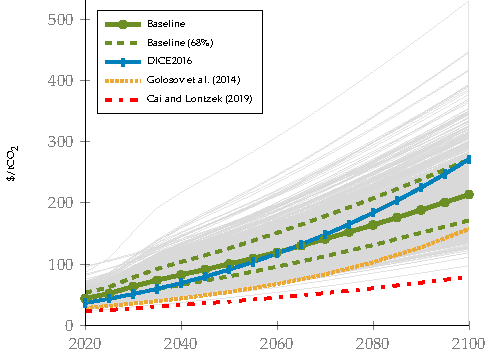
\includegraphics[width=0.5\textwidth]{images/fig_SCC.pdf} \newline\vspace{2ex}
\begin{minipage}{14cm}
\tiny\underline{Note:} The figure displays the social cost of carbon (SCC) on the vertical axis. The baseline model from \cite{jondeau2022environmental} is represented by a solid green line. Uncertainty interval, computed from 2,000 simulations using alternative parameter draws from the Metropolis-Hastings algorithm, are depicted by solid gray lines. Alternative SCC are also presented: (i) DICE2016 (solid blue with vertical markers), (ii) \cite{Golosov_et_al_2014} (orange dotted line), and (iii) \citealp{Cai&Lontzek19} with a benchmark calibration assuming 1.5\% total factor productivity growth (red dashed line).
\end{minipage}
\end{figure}%

%TCIMACRO{\TeXButton{Transition: Box Out}{\transboxout}}%
%BeginExpansion
\transboxout
%EndExpansion%
%TCIMACRO{\TeXButton{EndFrame}{\end{frame}}}%
%BeginExpansion
\end{frame}%
%EndExpansion
%

%TCIMACRO{\TeXButton{PAPER OUTLINE}{\begin{frame}{Outline}
%\tableofcontents\end{frame}}}%
%BeginExpansion
\begin{frame}{Outline}
\tableofcontents\end{frame}%
%EndExpansion


\section{The Optimal\ Control\ Problem}%

%TCIMACRO{\TeXButton{BeginFrame}{\begin{frame}}}%
%BeginExpansion
\begin{frame}%
%EndExpansion
%

%TCIMACRO{\QTR{frametitle}{Control Problem: the objective function}}%
%BeginExpansion
\frametitle{Control Problem: the objective function}%
%EndExpansion


\begin{itemize}
\item \textbf{Individual preferences.} Utility from consumption $u(c)$ with
$u^{\prime}(c)>0$ and $u^{\prime\prime}(c)<0$ (diminishing marginal utility).
We use CRRA:%
\[
u(c)=%
\begin{cases}
\dfrac{c^{1-\gamma}-1}{1-\gamma}, & \gamma\neq1,\\[0.6em]%
\log c, & \gamma=1,
\end{cases}
\qquad\gamma>0.
\]


\item \textbf{Aggregation and units.} Let $C_{t}$ be aggregate consumption
(trillion USD) and $L_{t}$ population (million). Per-capita consumption in
\emph{thousand USD} is
\[
c_{t}\;=\;1,000\times\frac{C_{t}}{L_{t}}.
\]
Instantaneous social welfare is $L_{t}\,u(c_{t})$.

\item \textbf{Intertemporal welfare.} With pure rate of time preference
$\rho>0$,%
\[
W_{t}=\sum_{i=0}^{\infty}\frac{L_{t+\Delta i}\,u(c_{t+\Delta i})}%
{(1+\rho)^{\Delta i}}.
\]

\end{itemize}

%

%TCIMACRO{\TeXButton{Transition: Box Out}{\transboxout}}%
%BeginExpansion
\transboxout
%EndExpansion%
%TCIMACRO{\TeXButton{EndFrame}{\end{frame}}}%
%BeginExpansion
\end{frame}%
%EndExpansion
%

%TCIMACRO{\TeXButton{BeginFrame}{\begin{frame}}}%
%BeginExpansion
\begin{frame}%
%EndExpansion
%

%TCIMACRO{\QTR{frametitle}{Control Problem: the solution toolkit}}%
%BeginExpansion
\frametitle{Control Problem: the solution toolkit}%
%EndExpansion


\textbf{Planner's problem.} Consider a government that chooses decisions
variables (savings/investment $S_{t}$ and abatement $\mu_{t}$) to maximize
\[
\max_{\{s_{t},\mu_{t}\}_{i\geq0}}\;\sum_{i=0}^{\infty}\frac{L_{t+\Delta
i}\,u(c_{t+\Delta i})}{(1+\rho)^{\Delta i}}\quad\text{{\small s.t. resource,
capital, ..}.}%
\]


How to solve the problem?

\begin{enumerate}
\item \textbf{Numerical solver:} use solver to find sequences $\left\{
S_{t},\mu_{t}\right\}  _{t=0}^{T}$ that maximizes objective.

\item \textbf{Ramsey solution:} maximize social welfare based on $N_{y}%
$\ equations and $N_{y}+N_{z}$ control variables.

\item \textbf{Dynamic programming:} use Bellman equation and value function
iterations or projections possibly with fancy neural networks.
\end{enumerate}

%

%TCIMACRO{\TeXButton{Transition: Box Out}{\transboxout}}%
%BeginExpansion
\transboxout
%EndExpansion%
%TCIMACRO{\TeXButton{EndFrame}{\end{frame}}}%
%BeginExpansion
\end{frame}%
%EndExpansion
%

%TCIMACRO{\TeXButton{BeginFrame}{\begin{frame}}}%
%BeginExpansion
\begin{frame}%
%EndExpansion
%

%TCIMACRO{\QTR{frametitle}{Control Problem: model summary (a recap)}}%
%BeginExpansion
\frametitle{Control Problem: model summary (a recap)}%
%EndExpansion


\begin{itemize}
\item \textbf{Exogenous variables} each driven by an exogenous process
(growth/decline path).%
\[
x_{t}=\{A_{t},\ \sigma_{t},\ \theta_{1,t},\ F_{t}^{EX},\ E_{t}^{\text{land}%
},\ L_{t}\}
\]


\item \textbf{Endogenous state/flow variables}%
\[
y_{t}=\{M_{t}^{AT},\ M_{t}^{UP},\ M_{t}^{LO},\ T_{t}^{AT},\ T_{t}^{LO}%
,\ Y_{t},\ K_{t},\ C_{t}\}
\]


\item \textbf{Decision variables (controls)}%
\[
z_{t}=\{\mu_{t},\ s_{t}\}
\]


\item \textbf{Horizon and time step:} $t\in\{2015,2020,2025,\ldots,T\}$,
$\Delta=5$ years (quinqennial).
\end{itemize}

%

%TCIMACRO{\TeXButton{Transition: Box Out}{\transboxout}}%
%BeginExpansion
\transboxout
%EndExpansion%
%TCIMACRO{\TeXButton{EndFrame}{\end{frame}}}%
%BeginExpansion
\end{frame}%
%EndExpansion
%

%TCIMACRO{\TeXButton{BeginFrame}{\begin{frame}}}%
%BeginExpansion
\begin{frame}%
%EndExpansion
%

%TCIMACRO{\QTR{frametitle}{Control Problem: a sketch of the numerical
%solution}}%
%BeginExpansion
\frametitle{Control Problem: a sketch of the numerical solution}%
%EndExpansion


\begin{itemize}
\item Because the social welfare is forward looking, the system is both
forward and backward looking as follows:%
\[
z_{t}=\arg\min_{\{s_{t},\mu_{t}\}_{i\geq0}}-\sum_{i=0}^{\infty}(1+\rho
)^{-\Delta i}L_{t+\Delta i}\,u(c_{t+\Delta i})
\]


\item When a sequence $\{z_{t+\Delta i}\}_{i=0}^{\infty}$ is found, one can
compute:
\begin{align*}
x_{t}  &  =g(x_{t-1}),\qquad\text{\ \ \ \ \ \ \ \ \ }g:\ \mathbb{R}^{N_{x}%
}\rightarrow\mathbb{R}^{N_{x}},\\[0.3em]
y_{t}  &  =f\big(y_{t-1},\,x_{t},\,z_{t}\big),\qquad f:\ \mathbb{R}^{N_{y}%
}\times\mathbb{R}^{N_{x}}\times\mathbb{R}^{2}\rightarrow\mathbb{R}^{N_{y}}.
\end{align*}


\item $x_{t}\in\mathbb{R}^{N_{x}}$: \textbf{exogenous variables}
($A_{t},\ \sigma_{t},\ \ldots,L_{t}$).

\item $y_{t}\in\mathbb{R}^{N_{y}}$: \textbf{endogenous states/flows}
($M_{t}^{AT},M_{t}^{UP},\ldots,Y_{t},K_{t}$).

\item $z_{t}=[\mu_{t},s_{t}]^{\prime}\in\mathbb{R}^{2}$: \textbf{decision
variables} (abatement, saving).
\end{itemize}

%

%TCIMACRO{\TeXButton{Transition: Box Out}{\transboxout}}%
%BeginExpansion
\transboxout
%EndExpansion%
%TCIMACRO{\TeXButton{EndFrame}{\end{frame}}}%
%BeginExpansion
\end{frame}%
%EndExpansion
%

%TCIMACRO{\TeXButton{BeginFrame}{\begin{frame}}}%
%BeginExpansion
\begin{frame}%
%EndExpansion
%

%TCIMACRO{\QTR{frametitle}{Control Problem: a sketch of the numerical
%solution}}%
%BeginExpansion
\frametitle{Control Problem: a sketch of the numerical solution}%
%EndExpansion


\begin{itemize}
\item \textbf{Idea.} Approximate the \textbf{infinite-horizon} objective with
a \textbf{finite} one. Let $\beta_{\Delta}\equiv(1+\rho)^{-\Delta}$. Because
$\lim_{i\rightarrow\infty}\beta_{\Delta}^{i}=0$, the tail contributes little.

\item \textbf{Pick the horizon $I^{\star}$ }so that the tail weight is below a
tolerance $\varepsilon$:
\[
\beta_{\Delta}^{\,I^{\star}}\leq\varepsilon\quad
%\Longrightarrow\quad I^{\star}\;\geq\;\Big\lceil\frac{\ln\varepsilon}{\ln\beta_{\Delta}}\Big\rceil.
\]
\emph{Trade-off:} smaller $I^{\star}$ $\Rightarrow$ faster solve but larger
truncation error.

\item \textbf{Finite-horizon problem }with $T=t+I^{\star}\Delta$, solve
\[
\max_{\{s_{t+i},\,\mu_{t+i}\}_{i=0}^{I^{\star}}}\;\sum_{i=0}^{I^{\star}}%
\beta_{\Delta}^{\,i}\,L_{t+i\Delta}\,u\!\left(  1000\,\times\frac
{C_{t+i\Delta}}{L_{t+i\Delta}}\right)  \;
\]%
\[
\text{s.t. dynamics (resource, capital, emissions, climate) and bounds.}%
\]

\end{itemize}

%

%TCIMACRO{\TeXButton{Transition: Box Out}{\transboxout}}%
%BeginExpansion
\transboxout
%EndExpansion%
%TCIMACRO{\TeXButton{EndFrame}{\end{frame}}}%
%BeginExpansion
\end{frame}%
%EndExpansion
%

%TCIMACRO{\TeXButton{BeginFrame}{\begin{frame}}}%
%BeginExpansion
\begin{frame}%
%EndExpansion
%

%TCIMACRO{\QTR{frametitle}{Control Problem: Two Policies}}%
%BeginExpansion
\frametitle{Control Problem: Two Policies}%
%EndExpansion


\begin{itemize}
\item The
%TCIMACRO{\TeXButton{green}{\color{green}}}%
%BeginExpansion
\color{green}%
%EndExpansion
mitigation policy%
%TCIMACRO{\TeXButton{black}{\color{black}}}%
%BeginExpansion
\color{black}%
%EndExpansion
:%
\begin{gather*}
\max_{\{s_{t+i},\,\mu_{t+i}\}_{i=0}^{I^{\star}}}\sum\nolimits_{i=0}^{I^{\star
}}\beta_{\Delta}^{\,i}\,L_{t+i\Delta}\,u\!\left(  1000\times\,\frac
{C_{t+i\Delta}}{L_{t+i\Delta}}\right)  \;\\
\text{s.t. dynamics (resource, capital, emissions, climate) and bounds.}%
\end{gather*}%
%TCIMACRO{\TeXButton{vspace}{\vspace{1.5ex}}}%
%BeginExpansion
\vspace{1.5ex}%
%EndExpansion


\item The\textit{
%TCIMACRO{\TeXButton{green}{\color{red}}}%
%BeginExpansion
\color{red}%
%EndExpansion
laisser-faire} /\ Business As Usual (BAU) policy%
%TCIMACRO{\TeXButton{black}{\color{black}}}%
%BeginExpansion
\color{black}%
%EndExpansion
:%
\begin{gather*}
\max_{\{s_{t+i},\}_{i=0}^{I^{\star}}}\sum\nolimits_{i=0}^{I^{\star}}%
\beta_{\Delta}^{\,i}\,L_{t+i\Delta}\,u\!\left(  1000\,\times\frac
{C_{t+i\Delta}}{L_{t+i\Delta}}\right)  \;\\
\text{s.t. dynamics (resource, capital, emissions, climate) and bounds.}\\
s.t.\text{ }\mu_{t}=0.03
\end{gather*}

\end{itemize}

%

%TCIMACRO{\TeXButton{Transition: Box Out}{\transboxout}}%
%BeginExpansion
\transboxout
%EndExpansion%
%TCIMACRO{\TeXButton{EndFrame}{\end{frame}}}%
%BeginExpansion
\end{frame}%
%EndExpansion
%

%TCIMACRO{\TeXButton{BeginFrame}{\begin{frame}}}%
%BeginExpansion
\begin{frame}%
%EndExpansion


\begin{center}
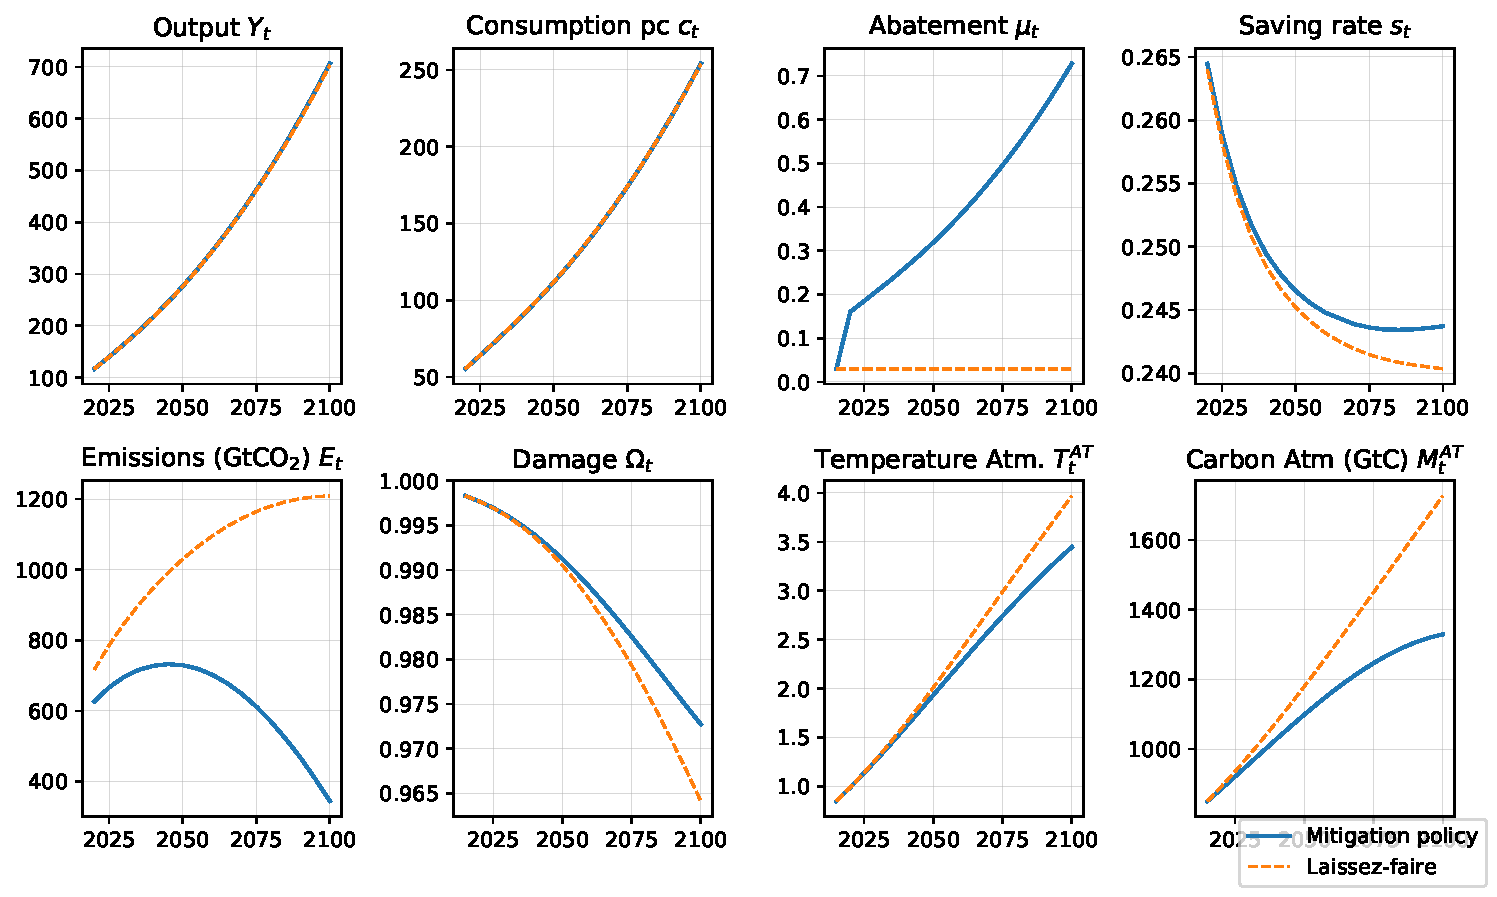
\includegraphics[clip,width=0.85\textwidth]{images/figure_1.pdf}\newline

Figure.\ Simulations under two policy scenarios
\end{center}

%

%TCIMACRO{\TeXButton{Transition: Box Out}{\transboxout}}%
%BeginExpansion
\transboxout
%EndExpansion%
%TCIMACRO{\TeXButton{EndFrame}{\end{frame}}}%
%BeginExpansion
\end{frame}%
%EndExpansion
%

%TCIMACRO{\TeXButton{BeginFrame}{\begin{frame}}}%
%BeginExpansion
\begin{frame}%
%EndExpansion


Some striking but controversial results from DICE:%
%TCIMACRO{\TeXButton{vspace}{\vspace{1.5ex}}}%
%BeginExpansion
\vspace{1.5ex}%
%EndExpansion


\begin{stepitemizewithalert}
\item \textquotedblleft Optimal\textquotedblright\ to warm the planet up to
3.3$%
%TCIMACRO{\U{b0}}%
%BeginExpansion
{{}^\circ}%
%EndExpansion
C;$%
%TCIMACRO{\TeXButton{vspace}{\vspace{1.5ex}}}%
%BeginExpansion
\vspace{1.5ex}%
%EndExpansion


\item Mitigation policy saves about 1\% of climate damage;%
%TCIMACRO{\TeXButton{vspace}{\vspace{1.5ex}}}%
%BeginExpansion
\vspace{1.5ex}%
%EndExpansion


\item Net zero emission optimal by 2130, 80 years later than in
Paris-Agreement;%
%TCIMACRO{\TeXButton{vspace}{\vspace{1.5ex}}}%
%BeginExpansion
\vspace{1.5ex}%
%EndExpansion


\item Main critic from DICE's policy output: those results have scientifically
grounded climate inaction in policy circles...%
%TCIMACRO{\TeXButton{vspace}{\vspace{1.5ex}}}%
%BeginExpansion
\vspace{1.5ex}%
%EndExpansion
\newline...\ but DICE has also the merit to set the climate issue to the
agenda of (macro-)economists.
\end{stepitemizewithalert}

%

%TCIMACRO{\TeXButton{Transition: Box Out}{\transboxout}}%
%BeginExpansion
\transboxout
%EndExpansion%
%TCIMACRO{\TeXButton{EndFrame}{\end{frame}}}%
%BeginExpansion
\end{frame}%
%EndExpansion


\section{The SSC\ in the Ramsey Problem}%

%TCIMACRO{\TeXButton{BeginFrame}{\begin{frame}}}%
%BeginExpansion
\begin{frame}%
%EndExpansion
%

%TCIMACRO{\QTR{frametitle}{Social cost of carbon}}%
%BeginExpansion
\frametitle{Social cost of carbon}%
%EndExpansion


\begin{stepitemizewithalert}
\item Why is it optimal to warm so much the planet according to DICE?%
%TCIMACRO{\TeXButton{vspace}{\vspace{1.5ex}}}%
%BeginExpansion
\vspace{1.5ex}%
%EndExpansion


\item An optimal carbon tax = how much the society is willing to pay to reduce
emissions (\$ per ton of carbon).%
%TCIMACRO{\TeXButton{vspace}{\vspace{1.5ex}}}%
%BeginExpansion
\vspace{1.5ex}%
%EndExpansion


\item This is usually referred to as the Social Cost of Carbon (SCC) in
literature.%
%TCIMACRO{\TeXButton{vspace}{\vspace{1.5ex}}}%
%BeginExpansion
\vspace{1.5ex}%
%EndExpansion


\item SCC reflects the society's gains and losses from implementing the carbon
tax.%
%TCIMACRO{\TeXButton{vspace}{\vspace{1.5ex}}}%
%BeginExpansion
\vspace{1.5ex}%
%EndExpansion


\item What is the model implied SCC? Let's use Ramsey problem!
\end{stepitemizewithalert}

%

%TCIMACRO{\TeXButton{Transition: Box Out}{\transboxout}}%
%BeginExpansion
\transboxout
%EndExpansion%
%TCIMACRO{\TeXButton{EndFrame}{\end{frame}}}%
%BeginExpansion
\end{frame}%
%EndExpansion
%

%TCIMACRO{\TeXButton{BeginFrame}{\begin{frame}}}%
%BeginExpansion
\begin{frame}%
%EndExpansion


The \cite{ramsey1927contribution} problem:%
\begin{align*}
&  \max_{\{c_{t},Y_{t},K_{t},T_{t},M_{t},\mu_{t},s_{t}\}}\sum_{i=0}^{\infty
}\beta_{\Delta}^{\,i}L_{t+\Delta i}\,u(c_{t+\Delta i})\\
&  +\beta_{\Delta}^{\,i}\lambda_{1,t+\Delta i}\left[  \left(  1-s_{t+\Delta
i}\right)  Y_{+\Delta it}\left(  1-\theta_{1,t+\Delta i}\mu_{t+\Delta
i}^{\theta_{2}}\right)  \Omega\left(  T_{t+\left(  i-1\right)  \Delta}\right)
-L_{t+\Delta i}c_{t+\Delta i}/1,000\right]  \\
&  +\beta_{\Delta}^{\,i}\lambda_{2,t+\Delta i}\left[  K_{t+\Delta i}-\left(
1-\delta_{K}\right)  K_{t+\left(  i-1\right)  \Delta}-s_{t+\Delta
i}Y_{t+\Delta i}\left(  1-\theta_{1,t+\Delta i}\mu_{t+\Delta i}^{\theta_{2}%
}\right)  \Omega\left(  T_{t+\left(  i-1\right)  \Delta}\right)  \right]  \\
&  +\beta_{\Delta}^{\,i}\lambda_{3,t+\Delta i}\left[  Y_{t+\Delta
i}-A_{t+\Delta i}K_{t+\left(  i-1\right)  \Delta}^{\gamma}L_{t+\Delta
i}^{1-\gamma}\right]  \\
&  +\beta_{\Delta}^{\,i}\lambda_{4,t+\Delta i}\left[  T_{t+\Delta i}-\Phi
_{T}T_{t+\left(  i-1\right)  \Delta}-\Xi_{T}F_{t+\Delta i}\left(  M_{t+\Delta
i}\right)  \right]  \\
&  +\beta_{\Delta}^{\,i}\lambda_{5,t+\Delta i}\left[  M_{t+\Delta i}-\Phi
_{M}M_{t+\left(  i-1\right)  \Delta}-\Xi_{M}\left(  \sigma_{t+\Delta i}\left(
1-\mu_{t+\Delta i}\right)  Y_{t+\Delta i}+E_{t+\Delta i}^{\text{land}}\right)
\right]
\end{align*}


\textbf{Summary:} optimal control problem with $7$ control variables, $5$
constraints $\rightarrow12$ variables/equations.

(note that climate variables include more equations + Lagrangian multipliers)%

%TCIMACRO{\TeXButton{Transition: Box Out}{\transboxout}}%
%BeginExpansion
\transboxout
%EndExpansion%
%TCIMACRO{\TeXButton{EndFrame}{\end{frame}}}%
%BeginExpansion
\end{frame}%
%EndExpansion
%

%TCIMACRO{\TeXButton{BeginFrame}{\begin{frame}}}%
%BeginExpansion
\begin{frame}%
%EndExpansion


\begin{itemize}
\item Recall that compact form for climate block with
\[
T_{t}=[T_{t}^{AT},T_{t}^{LO}]^{\top}\text{ and }M_{t}=[M_{t}^{AT},M_{t}%
^{UP},M_{t}^{LO}]^{\top}%
\]


\item The corresponding multipliers:%
\[
\lambda_{4,t}=[\lambda_{5,t}^{AT},\lambda_{5,t}^{LO}]^{\top}\text{ \ and
}\lambda_{5,t}=[\lambda_{5,t}^{AT},\lambda_{5,t}^{UP},\lambda_{5,t}%
^{LO}]^{\top}%
\]


\item Damages and forcing functions as function of vectors $T_{t}$ and
$M_{t}:$
\begin{align*}
\Omega\left(  T_{t}\right)    & =1/\left(  1+a_{2}\left(  T_{t}^{AT}\right)
^{2}\right)  \\
F_{t}\left(  M_{t}\right)    & =\eta\ \log\left(  M_{t}^{AT}/M_{1750}\right)
/\log(2)+F_{t}^{EX}%
\end{align*}


\item Corresponding gradients:
\begin{align*}
\nabla_{T}\Omega\left(  T_{t}\right)    & =\left[
\begin{tabular}
[c]{ll}%
$-\Omega\left(  T_{t}\right)  ^{2}2a_{2}\left(  T_{t}^{AT}\right)  $ & $0$%
\end{tabular}
\right]  ^{\top}\\
\nabla_{M}F\left(  M_{t}\right)    & =\left[
\begin{tabular}
[c]{lll}%
$\eta/(M_{t}^{AT}\ln2)$ & $0$ & $0$%
\end{tabular}
\right]  ^{\top}%
\end{align*}

\end{itemize}%

%TCIMACRO{\TeXButton{Transition: Box Out}{\transboxout}}%
%BeginExpansion
\transboxout
%EndExpansion%
%TCIMACRO{\TeXButton{EndFrame}{\end{frame}}}%
%BeginExpansion
\end{frame}%
%EndExpansion


%

%TCIMACRO{\TeXButton{BeginFrame}{\begin{frame}}}%
%BeginExpansion
\begin{frame}%
%EndExpansion
%

%TCIMACRO{\QTR{frametitle}{Social cost of carbon}}%
%BeginExpansion
\frametitle{Social cost of carbon}%
%EndExpansion


\begin{stepitemizewithalert}
\item Get back to FOCs of the Ramsey-planner:%
\begin{align*}
T_{t} &  :\lambda_{4,t}=\beta_{\Delta}\left[  \Phi_{T}^{\top}\lambda
_{4,t+\Delta}+\lambda_{2,t+\Delta}s_{t+\Delta}Y_{t+\Delta}\left(
1-\theta_{1,t+\Delta}\mu_{t+\Delta}^{\theta_{2}}\right)  \nabla_{T}%
\Omega\left(  T_{t}\right)  \right]  \\
M_{t} &  :\lambda_{5,t}=\beta_{\Delta}\left[  \Phi_{M}^{\top}\lambda
_{5,t+\Delta}+\left(  \Xi_{T}^{\top}\lambda_{4,t+\Delta}\right)  \nabla
_{M}F\left(  M_{t}\right)  \right]
\end{align*}
$\lambda_{5,t}$ ($\lambda_{4,t}$) is the marginal loss from carbon
(temperature) increase in each climate box.%
%TCIMACRO{\TeXButton{vspace}{\vspace{1.5ex}}}%
%BeginExpansion
\vspace{1.5ex}%
%EndExpansion


\item SCC expresses the social loss into numeraire equivalents (here
consumption):%
\[
SSC_{t}=-1000\times\lambda_{5,t}^{AT}/\lambda_{1,t}\simeq-1000\times\left(
\partial W_{t}/\partial M_{t}^{AT}\right)  /\left(  \partial W_{t}/\partial
C_{t}\right)
\]
where $\lambda_{1,t}$\ is marginal utility of consumption while $\lambda
_{5,t}^{AT}$ measures the planner's value for a marginal change in atmospheric
carbon.%
%TCIMACRO{\TeXButton{vspace}{\vspace{1.5ex}}}%
%BeginExpansion
\vspace{1.5ex}%
%EndExpansion

\end{stepitemizewithalert}

%

%TCIMACRO{\TeXButton{Transition: Box Out}{\transboxout}}%
%BeginExpansion
\transboxout
%EndExpansion%
%TCIMACRO{\TeXButton{EndFrame}{\end{frame}}}%
%BeginExpansion
\end{frame}%
%EndExpansion
%

%TCIMACRO{\TeXButton{BeginFrame}{\begin{frame}}}%
%BeginExpansion
\begin{frame}%
%EndExpansion


\begin{center}
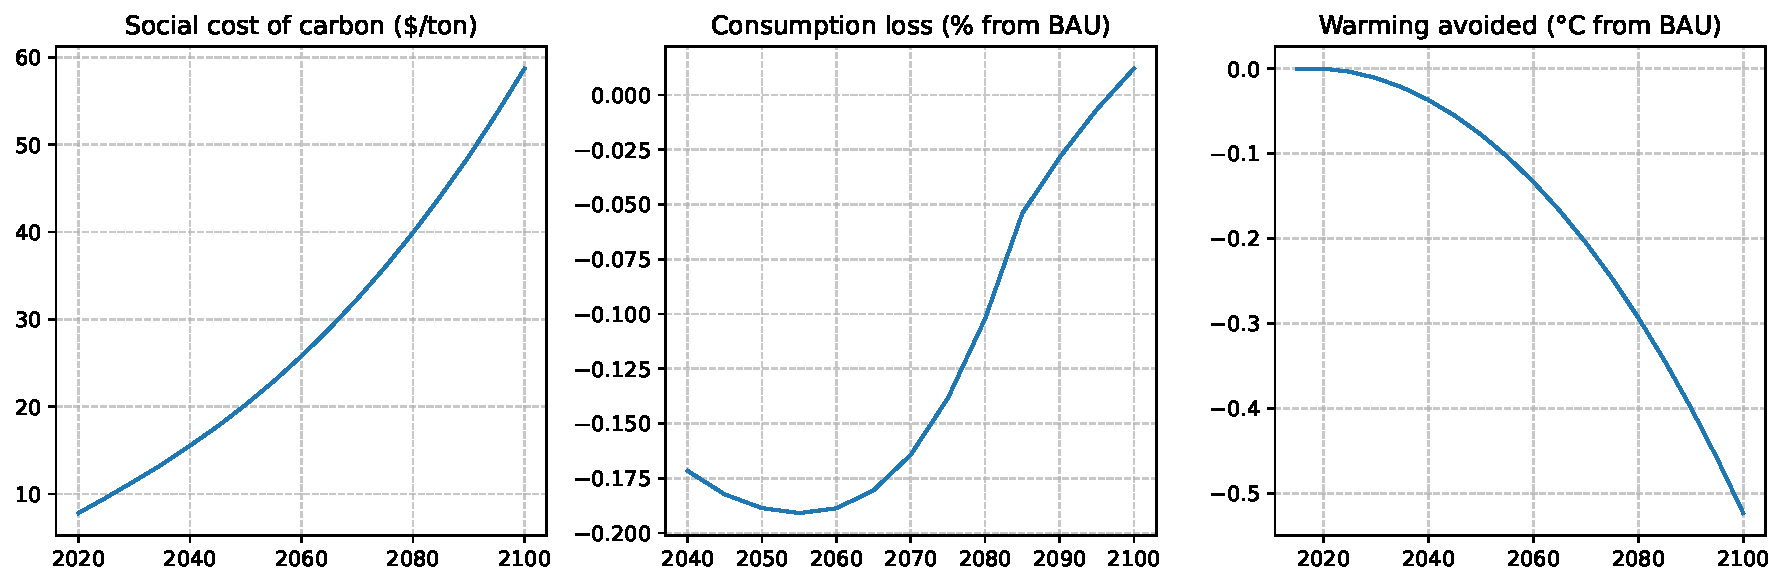
\includegraphics[width=0.68\textwidth]{images/figure_3.pdf}\newline
\end{center}

\begin{stepitemizewithalert}
\item SCC reflect the planner's relative gains in terms of welfare from
controlling $M_{t}$ against its consumption losses $C_{t}$ from such action;%
%TCIMACRO{\TeXButton{vspace}{\vspace{1.5ex}}}%
%BeginExpansion
\vspace{1.5ex}%
%EndExpansion


\item Optimal to cut consumption now by 0.2\% in order to avoid 0.55$%
%TCIMACRO{\U{b0}}%
%BeginExpansion
{{}^\circ}%
%EndExpansion
C$ of warming in 2100;%
%TCIMACRO{\TeXButton{vspace}{\vspace{1.5ex}}}%
%BeginExpansion
\vspace{1.5ex}%
%EndExpansion


\item As well off between scenarios by 2090 on current consumption grounds
(but not in welfare terms).
\end{stepitemizewithalert}

%

%TCIMACRO{\TeXButton{Transition: Box Out}{\transboxout}}%
%BeginExpansion
\transboxout
%EndExpansion%
%TCIMACRO{\TeXButton{EndFrame}{\end{frame}}}%
%BeginExpansion
\end{frame}%
%EndExpansion
%

%TCIMACRO{\TeXButton{BeginFrame}{\begin{frame}}}%
%BeginExpansion
\begin{frame}%
%EndExpansion
%

%TCIMACRO{\QTR{frametitle}{Social cost of carbon}}%
%BeginExpansion
\frametitle{Social cost of carbon}%
%EndExpansion


\begin{stepitemizewithalert}
\item How to retrieve the SCC if we don't have any lagrangian multiplier?
\end{stepitemizewithalert}

\begin{itemize}
\item One can use the firm's static problem (given output $Y_{t}$):
\[
\min_{\mu_{t}\in\lbrack0,1]}\;\underbrace{\theta_{1,t}\,\mu_{t}^{\theta_{2}%
}\,Y_{t}}_{\text{abatement cost}}\;+\;\tau_{t}\,\underbrace{\sigma_{t}%
(1-\mu_{t})\,Y_{t}}_{\text{taxed residual emissions}}.
\]


\item First-order condition in $\mu_{t}$:
\[
\theta_{2}\,\theta_{1,t}\,\mu_{t}^{\theta_{2}-1}Y_{t}\;=\;\tau_{t}\,\sigma
_{t}\,Y_{t}\quad\Rightarrow\quad
\boxed{\;\tau_t \;=\; \frac{\theta_2\,\theta_{1,t}}{\sigma_t}\,\mu_t^{\theta_2-1}\;}
\]


\item This \ tax is in trillion USD\ per gigatonne carbon.\ The carbon tax
$\tau_{t}^{\$}$ in US\$/tCO$_{2}$:
\[
\tau_{t}^{\$}=\frac{10^{12}}{10^{9}}\times\tau_{t}=1,000\times\tau_{t}%
\]
as $1GtC=10^{9}$ and $1$ $trillion$ $\$=10^{12}$.
\end{itemize}%

%TCIMACRO{\TeXButton{Transition: Box Out}{\transboxout}}%
%BeginExpansion
\transboxout
%EndExpansion%
%TCIMACRO{\TeXButton{EndFrame}{\end{frame}}}%
%BeginExpansion
\end{frame}%
%EndExpansion


%TCIMACRO{\TeXButton{FRAME}{\bibliographystyle{apalike}
%\bibliography{lucas_romie}}}%
%BeginExpansion
\bibliographystyle{apalike}
\bibliography{lucas_romie}%
%EndExpansion

\end{document}
